\documentclass[a4paper, 10pt, final, garamond]{book}
\usepackage{cours-preambule}
\graphicspath{{./figures/}}

\makeatletter
\renewcommand{\@chapapp}{Contr\^ole de connaissances}
\makeatother

% \toggletrue{student}
% \toggletrue{corrige}
\renewcommand{\mycol}{black}
% \renewcommand{\mycol}{gray}

\begin{document}
\setcounter{chapter}{27}

\settype{enon}
\settype{solu}

\chapter{Second principe, machines et changements d'états\ifstudent{~(18')}}

\vspace{-20pt}
\begin{tcn}(data)<lftt>{Données}
	$\Delta{S}\sup{cond} = mc \ln \frac{T_f}{T_i}$
	\hspace{20pt}
	et
	\hspace{20pt}
	$\Delta{S}\sup{G.P.} =
		C_V \ln \frac{T_f}{T_i} + nR \ln \frac{V_f}{V_i} =
		C_P \ln \frac{T_f}{T_i} - nR \ln \frac{P_f}{P_i} =
		C_V \ln \frac{P_f}{P_i} + C_P \ln \frac{V_f}{V_i}$
	\vspace{-15pt}
\end{tcn}

\begin{enumerate}[label=\sqenumi]
	\item[n]{7}
	Soit un gaz parfait passant de l'état initial $I$ $(T_i, P_i, V_i = V_0)$ à un
	état final $f$ $(T_f, P_f, V_f = V_0)$ en le mettant en contact avec un
	thermostat de température $T\ind{ext} = T_f$. \textbf{Déterminer
		$\Delta{S}$, $S\ind{ech}$ et $S\ind{cr}$ en fonction de $n$, $R$, $\gamma$
		et $x = \frac{T_i}{T_f}$}. Conclure sur la nature réversible ou non de la
	transformation par un raisonnement mathématique.
	\smallbreak
	\begin{isd}
		\psw{%
			\begin{gather*}
				\Delta{S} =
				C_V \ln \frac{T_f}{T_i} +
				\underbracket[1pt]{nR \ln \frac{V_f}{V_i}}_{=0}
				\Ra
				\boxed{\Delta{S} \stm{=} -\frac{nR}{\gamma-1} \ln (x)}
				\\\beforetext{Or}
				S\ind{ech} \stc"\footnotesize"{\stm(un){=}}{monoT.} \frac{Q}{T_f}
				\qqet
				\Delta{U} \stc"\footnotesize"{=}{isoV.} Q + \cancel{W}
				\\\Lra
				\frac{nR}{\gamma-1}(T_f-T_i) \stm{=} Q
				\Lra
				\boxed{
					S\ind{ech} \stm{=}
					\frac{nR}{\gamma-1} \left(1 - x\right)
				}
			\end{gather*}
			% \vspace{-15pt}
		}%
		\tcblower
		\psw{%
			\begin{align*}
				\beforetext{Or}
				\Delta{S}         & \stm{=} S\ind{ech} + S\ind{cr}
				\\\Lra
				\Aboxed{S\ind{cr} & = \Delta{S} - S\ind{ech} = C_V (x - 1 - \ln x)}
			\end{align*}
			Or, $\forall x \in \Rb\setminus\{1\},\, x-1 > \ln x$ \pt{1} donc $\boxed{S\ind{cr} > 0}$
			(sauf pour $T_i = T_f$ inutile)~: elle est \textbf{irréversible}. \pt{1}
		}%
		% \vspace{-15pt}
		% \begin{center}
		% 	\sswitch{
		% 		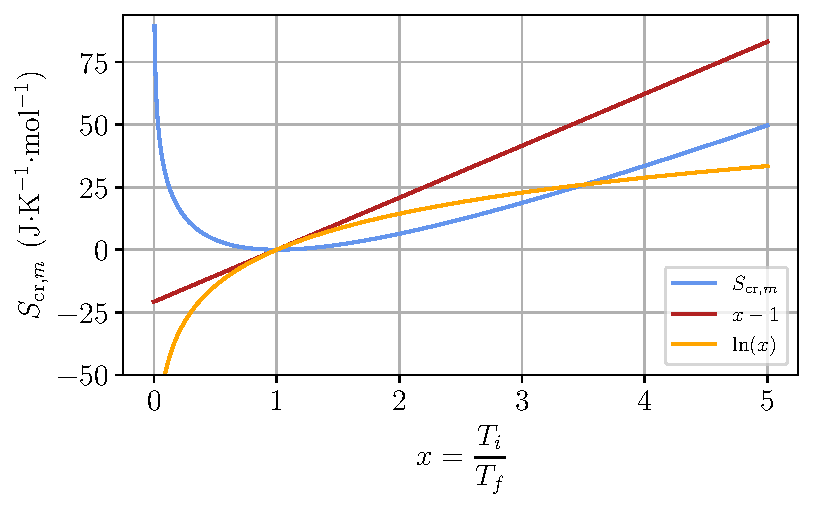
\includegraphics[width=.7\linewidth, draft=true]{DSappl_1}
		% 	}{
		% 		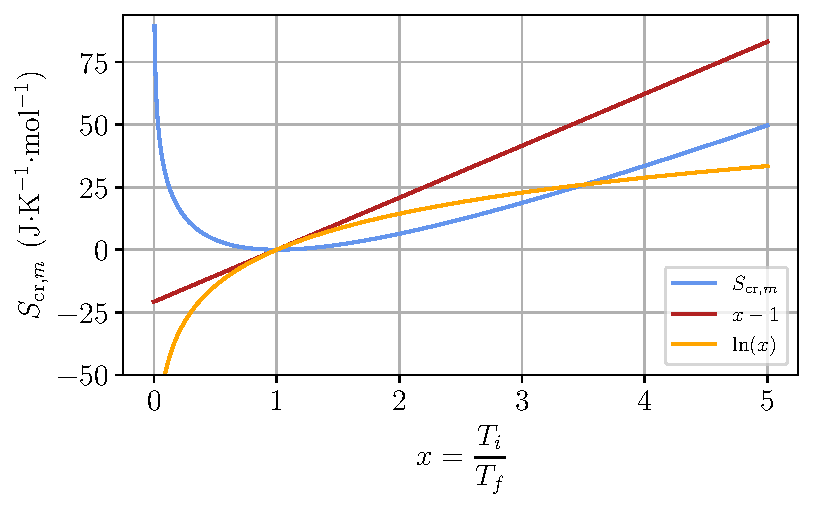
\includegraphics[width=.7\linewidth]{DSappl_1}
		% 	}
		% 	\vspace{-15pt}
		% \end{center}
	\end{isd}
	\item[n]{9}
	Présenter le réfrigérateur~: schéma de fonctionnement, signe algébrique des
	échanges, but, sources, production coût et pertes, et démontrer l'efficacité
	de \textsc{Carnot} du frigo.
	\smallbreak
	\begin{isd}[righthand ratio=.3]
		\begin{isd}
			\begin{itemize}
				\item[bl](\pt{1}){But}: \psw{\textbf{Refroidir source froide}}
				\item[bl](\pt{1}){\color{red}Source chaude}: \psw{atmosphère}
				\item[b]{\color{blue}Source froide}: \psw{aliments}
			\end{itemize}
			\begin{tabularx}{\linewidth}{YYY}
				\tikzmark{PR}%
				\textbf{Produc$^\circ$} &
				\textbf{Coût}           &
				\textbf{Perte}
				\\
				\psw{$Q_F$}             &
				\psw{$W$}               &
				\psw{$Q_C$}
			\end{tabularx}
			\tcblower
			\begin{center}
				\sswitch{
					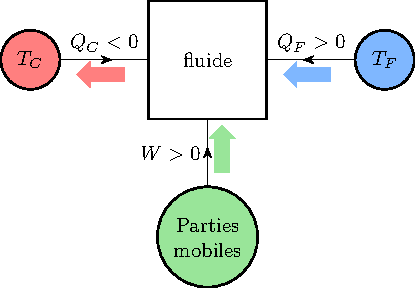
\includegraphics[width=\linewidth, draft=true]{refrig_dth}
				}{
					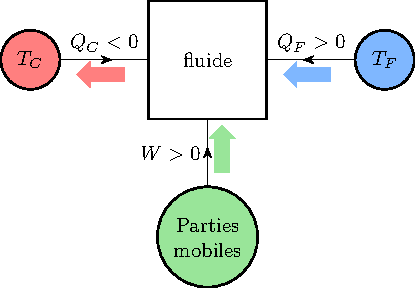
\includegraphics[width=\linewidth]{refrig_dth}
				}
				\vspace{-15pt}
				\captionof*{figure}{Schéma frigo.\protect \pt{1}\psw{ + }\protect\pt{1}}
			\end{center}
		\end{isd}
		\tcblower
		\psw{%
			\begin{DispWithArrows*}[fleqn, mathindent=-5pt, groups]
				e &\stm{=}
				\frac{Q_F}{W} \stm{=}
				-\frac{Q_F}{Q_C+Q_F}
				\\\Lra
				e &= -\frac{1}{1+\frac{Q_C}{Q_F}}
				\Arrow{$\frac{Q_C}{T_C} \stm[-1]{\leq} -\frac{Q_F}{T_F}$\\Or,
					$Q_F > 0$\\$1+\frac{Q_C}{Q_F} \leq 1 - \frac{T_C}{T_F}$}
				\\\Lra
				e &\leq - \frac{1}{1 - \frac{T_C}{T_F}}
				\\\Lra
				e &\leq \boxed{\frac{T_F}{T_C-T_F} \stm{=} e_C}
			\end{DispWithArrows*}
		}%
	\end{isd}
	\tikz[remember picture, overlay]
	\node[left] at ([shift={(-6pt,0pt)}]pic cs:PR) {\pt{1}};
	\item[n]{4}
	Énoncer et démontrer le théorème des moments, en vous appuyant sur une
	isotherme d'\textsc{Andrews} que vous tracerez.
	\smallbreak
	\begin{isd}
		\psw{%
			Soit $V_g$ et $V_{\ell}$ les volumes de gaz et de liquide, et $V = V_g +
				V_{\ell}$ le volume total.
			\begin{DispWithArrows*}
				v &= \frac{V_g}{m} + \frac{V_{\ell}}{m}
				\Arrow{$v = V/m$\\$\Lra V = mv$}
				\\\Lra
				v &\stm[-1]{=} \frac{m_gv_g}{m} + \frac{m_{\ell}v_{\ell}}{m}
				\Arrow{$x_g = m_g/m$}
				\\\Lra
				v &= x_gv_g + x_{\ell}v_{\ell}
				\Arrow{$x_g = 1-x_{\ell}$}
				\\\Lra
				v &\stm{=} (1-x_{\ell})v_g + x_{\ell}v_{\ell}
				\\\Lra
				x_{\ell} &= \frac{v_g-v}{v_g-v_{\ell}} = \frac{MG}{LG}
				\\\stm{\text{et}} \quad
				x_g &= \frac{v-v_{\ell}}{v_g-v_{\ell}} = \frac{LM}{LG}
				\qed
			\end{DispWithArrows*}
		}%
		\tcblower
		\begin{center}
			\sswitch{
				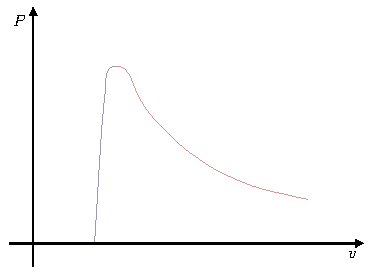
\includegraphics[width=\linewidth]{Pv_moment-stud}
			}{
				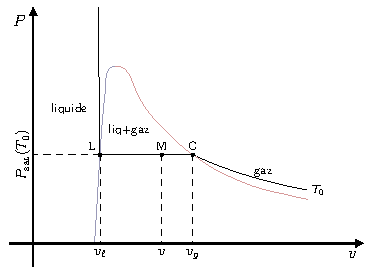
\includegraphics[width=\linewidth]{Pv_moment}
			}
			\vspace{-15pt}
			\captionof{figure}{Schéma théorème des moments.\protect \pt{1}}
		\end{center}
	\end{isd}
\end{enumerate}
\vspace{-15pt}
\ifstudent{
	\begin{tikzpicture}[remember picture, overlay]
		\node[anchor=north west, align=left]
		at ([shift={(1.4cm,0)}]current page.north west)
		{\\[5pt]\Large\bfseries Nom~:\\[10pt]\Large\bfseries Prénom~:};
		\node[anchor=north east, align=right]
		at ([shift={(-1.5cm,-17pt)}]current page.north east)
		{\Large\bfseries Note~:\hspace{1cm}/20};
	\end{tikzpicture}
}
\end{document}
